%% pcamaril_idi_V_report.tex
%% V1.0
%% 2021/02/28
%% by Victor Rodriguez
%%

\documentclass[]{PhDEngScITESO-R}

\graphicspath{ {img/} }

\usepackage{xr}

% We suggest the use of this extended package of graphics.
\usepackage{graphicx}
\usepackage{amssymb}
% Package that allow us to have subcaptions on images and tables.
\usepackage{caption}
\usepackage{subcaption}
% Package for design and management of plots.
\usepackage{tikz-network}
\usepackage{tikz,pgfplots}
\usetikzlibrary{shapes.geometric, arrows}
\usepackage{pgfplots}
\pgfplotsset{compat=1.16}
\usepackage{cite}
\usepackage[redeflists]{IEEEtrantools}
\usepackage{multirow}
\usepackage{booktabs}
\usepackage{graphicx}

\graphicspath{ {./img/} }

%%% HELPER CODE FOR DEALING WITH EXTERNAL REFERENCES
\usepackage{xr}
\makeatletter
\newcommand*{\addFileDependency}[1]{
  \typeout{(#1)}
  \@addtofilelist{#1}
  \IfFileExists{#1}{}{\typeout{No file #1.}}
}
\makeatother

\newcommand*{\myexternaldocument}[1]{
    \externaldocument{#1}
    \addFileDependency{#1.tex}
    \addFileDependency{#1.aux}
}
%%% END HELPER CODE


\myexternaldocument{PhDEngScITESO-YY-NN-RF}

% just to see what's happening
\listfiles

\begin{document}
	% Report title
	\bstctlcite{IEEEexample:BSTcontrol}
	\title{Characterization Of Benchmarks Using instructions histograms from pre-silicon virtual platforms }
	
	% Information of the PhD student and Report 
	\author{Victor Manuel Rodr\'{i}guez Bahena, Jose Luis Pizano, and Omar Longoria} 
	\reportid{PhDEngScITESO-21-XX}
	\reportYear{2022}
	\reportDate{Deccember, 2022}
	\itesoshield{iteso.png}
	
	\thanks{Authors thanks to National Council of Science and Technology for the
	scholarship No. 1143158 provided to this research.}
	
	\maketitle
	\begin{IEEEkeywords}
	SPEC CPU2017;  Characterization;  Analysis; Benchmarks
	\end{IEEEkeywords}


\begin{abstract}

The increasing complexity of  new CPU microarchitectures and SW applications makes the architectural simulator models extremely time-consuming. Simulators must manage massive numbers of instructions to simulate workloads that represent real applications. Although hardware evaluations benefit from this, using architectural simulators for such large numbers of instructions becomes infeasible, and executing the simulations in parallel results in a huge equipment cost. One way to solve this problem is by using reduced input sets instead of complete reference input sets. The ideal reduced input set has less instruction but produces program behavior comparable to the real application reference input set. This research study proposes a methodology that reliably quantifies program behavior similarity. With this methodology is possible to create new reduced input sets that result in program behavior similar to the previously executed workloads with more than 80\% accuracy and reduce pre-silicon simulation time by up to 7X. 

\end{abstract}
	
\section{Introduction}

Detailed pre-silicon analysis and verification of new features incorporated in new microprocessors often require the use of Register-transfer level (RTL) and virtual platform simulators. While the results of such studies can be very valuable, this approach is both slow and complex, resulting in extreme constraints on the maximum size of workloads that can be studied. because of this exists the microbenchmarks, according to \cite{Microbenchmark} a microbenchmark is either a program or routine to measure and test the performance of a single component or task. Microbenchmarks are used to measure simple and well-defined quantities such as elapsed time, rate of operations, bandwidth, or latency. Typically, microbenchmarks were associated with the testing of individual software subroutines or lower-level hardware components such as the CPU for a short period of time. Although microbenchmarks can be used for  pre-silicon analysis and verification, it is also desirable to characterize real-world workloads to find the minimum set of workloads that represent the highest amount of verification coverage.

Workload characterization represents an important step in designing future computer systems and it influences the design at all system levels from the hardware platforms to operating systems. A full understanding of workload properties and the way they execute sheds light on resource utilization and it can guide performance optimization at both the hardware and software levels. In addition, knowing the run time characteristics of an application is useful when making important decisions about hardware resource allocation. There is a need to know details about the structure and the properties of an application to understand the reasons for low run-time performance on hardware platforms. 

This work used a mix of workloads focused on : 
\begin{itemize}
\item Machine learning
\item In-memory data structure database
\item SPEC 2017 tests suite workloads.
\end{itemize}

 Each one of these workloads was executed through the virtual platform functional simulator (Simics \cite{Aarno}). Simics generates the histograms of instructions executed during the workload simulation. That will be the base of the methodology proposed by this work, to cluster the workloads by their similar instructions set executed. 

\subsection{Pre silicon Virtual Platform }

A virtual platform (VP) is a model of a hardware system that can run the same software as the hardware it models. The VP is simulated on a host computer that may be different from the hardware modeled by the virtual platform. A VP is not limited to modeling a single processor or board but can represent anything from a basic board with only a processor and memory to a complete system made up of network-connected boards, chassis, racks, and models of physical systems. Full-system simulation (FSS) is a term commonly used to describe these kinds of simulators \cite{Aarno} \cite{Yang}

The VP is useful for a part of the CPU development known as pre-silicon. During the pre-silicon process, engineers test devices in a virtual environment with simulation and emulation tools. In contrast, post-silicon validation tests occur on actual devices running at speed in commercial, real system boards. Post-silicon validation is used to detect and fix bugs in integrated circuits and systems after manufacture.

The main property of a pre-silicon virtual platform is its ability to run  software that will finally run on the post-silicon hardware system fast enough to be useful for software developers. Such software includes low-level firmware and boot loaders, hypervisors, operating systems, drivers, middleware, and applications. Therefore, the virtual platform accurately models the aspects of the real system that are relevant for software, such as histograms of the CPU instruction sets executed, device registers, memory maps, interrupts, and the functionality of the different devices. All these metrics provided by the virtual platform provide a set of tools for SW developers to release software long before the first silicon appears. At the same time, the CPU architects can validate the quality of their designs using the virtual platform earlier in the product life cycle.

It is important to highlight that the main limitation of the virtual platform is its lack of  modeling the detailed implementation of  hardware, such as internal buses, clocks, pipelines, and caches. For those metrics is necessary to use a cycle-accurate simulator such as Sniper \cite{sniper}

Despite all the features provided by the virtual platform simulators the increasing complexity of both microarchitectures and SW applications make these simulators very time-consuming. Simulators must execute huge numbers of instructions to create a workload representative of real applications. Using Virtual Platforms simulators for such large numbers of instructions becomes infeasible. 

According to \cite{Eeckhout}, pre-silicon simulation of workloads suites can represent  weeks of simulation, extending the time to market. Running the simulations in parallel results in a huge equipment cost. To solve this problem, the authors propose a subset of workloads that represent the most used suites of benchmarks that represent contemporary applications. One of these is the one created by the CPU design domain Standard Performance Evaluation Corporation (SPEC).

\subsection{SPEC CPU\textregistered\   2017}

The SPEC has released the SPEC CPU\textregistered\  suite since 1992. These benchmarks have become the standard for any researcher or commercial entity wishing to benchmark their architecture or design against existing ones. The latest release of the SPEC CPU\textregistered\ suite was released in June 2018 \cite{Singh}. SPEC CPU\textregistered\  2017 retains several benchmarks from the previous releases but has also added many new ones to reflect the changing nature of industry applications. The new suite is expected to become mainstream for simulation-based design and optimization research for next-generation processors, memory subsystems, and compilers.

\subsection{Machine learning workloads}

Data centers and cloud service providers are rapidly deploying Machine Learning applications (ML) to carry out a wide variety of learning tasks, such as speech recognition, natural language processing, and computer vision. As the training and inference tasks become increasingly complex, ML  workloads  demand  higher  computing  and  memory  capabilities.  For this experiment, the machine learning workloads used are

\begin{itemize}
\item ResNet-101 : Convolutional neural network that is 101 layers deep \cite{Zhang}.  
\item ResNet-50 : Convolutional neural network that is 50 layers deep
\item benchdnn : Correctness verification and performance benchmarking tool for the primitives provided by oneDNN ML library. \cite{Goli}
\end{itemize}

\subsection{Memtier workloads}

Memtier benchmark is a command line utility developed by Redis Labs for load generation and benchmarking No SQL key-value databases \cite{Alami}. The key-value databases work by keeping an in-memory data structure that is mapped to the data stored on disk. RAM is much faster than accessing data from disk so most databases will have some sort of algorithm to keep frequently accessed data in RAM and only fallback to disk if the index isn't already stored in memory.

The primary benefit of key-value databases and No SQL databases, in general, is the scalability they provide compared to relational databases. Databases typically become the primary bottleneck for software. Being able to abstract the basic operations of a database and focus on writing code that drove business value demanded by many tech companies is why the usage of key-value databases has grown so fast.

\section{Related works}

In the recent work \cite{Chishti}, authors present a  simulation infrastructure,  which implements a detailed memory profiling of deep neural network (DNN) workloads in a full-system simulation environment.  In this paper,  the authors report the key findings from memory characterization analysis of five popular DNNs implemented in the widely used  TensorFlow framework. 

One of the first results of this work was the breakdown of execution cycles spent in computing, memory, and synchronization operations for DNN workloads. Memory accesses constitute a significant portion of execution time, ranging from 25\% to 40\%, across the workloads analyzed. This memory characterization analysis demonstrates that the memory subsystem is one of the key bottlenecks for DNN performance scaling. Authors expect the memory system bottleneck to become more critical for DNN workloads in the future due to two main reasons. First, processors are incorporating hardware customization and  ISA  extensions to improve raw compute throughput (Multiply-adds per second), which reduces compute stall cycles. Second, future trends in DNNs are likely to put more pressure on on-chip cache capacity and memory bandwidth. This work requires the use of an interval simulation system (Sniper).

An interval simulation (IS) system is a simulation approach for simulating multi-core and multiprocessor systems. Interval simulation leverages an analytical model to an abstract core by driving the timing simulation of an individual core without the detailed tracking of individual instructions through the core's pipeline stages. Authors in \cite{Carlson} conclude that interval simulation and Sniper are useful complements in the toolbox of architects for simulating the performance of high-performance multi-core and many-core systems.

Despite the accuracy of IS systems are necessary that the simulation development teams support new ISA of incoming CPUs, which means a dependency in the development approach that virtual platform validation was addressing. Also, the execution time of Interval simulation systems such as Sniper can vary depending on the workload under analysis. In the point of cloud workloads, it could take days to execute. 

Some studies like \cite{Cheveresan} perform instruction decomposition showing important results that contradict the traditional way of characterizing the performance of applications. A similar paper \cite{Rupnow} provides an instruction classification breakdown of SPEC-FP 20008 and an internal benchmark suite. Adding more instruction kind categories like the ones provided in this work might provide a more accurate characterization

\section{Methodology}
\label{sec:Methodology}

The methodology consists of these next steps:

\begin{itemize}
 \item Collecting histograms of microbenchmarks
 \item Instructions decomposition
 \item Dimensionality reduction by principal component analysis (PCA)
 \item Unsupervised clustering by K-Means algorithm.
 \item Validate the accuracy of clustering
\end{itemize}

\subsection{Collecting histograms of microbenchmarks}
\label{subsec: Instructions decomposition }

Simics provides the capability to collect the histograms of instructions retired by the VP during the execution of the application or micro benchmark under analysis. The information is saved as a comma-separated value file with two columns: mnemonic and count. The mnemonic column has all the instructions executed and the count column shows how many times each instruction was executed. The user of Simics can define the moment when to start to capture the instructions histogram and when to stop the capture of instructions. Is not possible to isolate only the instructions for the processes related to the application, the Simics instructions histogram include all the operating system process executed at the same time as the application under analysis is being executed.

\subsection{Instructions decomposition}
\label{subsec: Instructions decomposition }

 Instruction decomposition provides critical data about the instruction mix of an application and represents an important step in functional and performance analysis. Each workload contains multiple instructions, and each one of them belongs to a specific kind of instruction. The instruction could be characterized in multiple categories, for example, the one suggested by \cite{Daniel}:

 \begin{itemize}
 \item Arithmetic and logic
 \item Memory ( Store)
 \item Stack
 \item Control Flow and condition.
 \item Prefix
 \item System and I/O
\end{itemize}

This study is going to use three more simple kinds of instructions described in Table \ref{table:1}. With this instruction, deposition is possible to see the characteristics of each histogram of the executed tests.

\subsection{ Dimensionality reduction }
\label{subsec:  Dimensionality reduction  }

Data analysis methods are essential for analyzing the ever-growing massive quantity of high-dimensional data. PCA is a statistical procedure that allows you to summarize the information contained in large data tables utilizing a shorter set of summary indices that can be more easily pictured and studied. PCA today is one of the most popular multivariate statistical techniques and is used in very broad areas such as meteorology, image processing, genomics analysis, and information retrieval.  The most important use of PCA is to represent a multivariate data table as a smaller set of variables (summary indices) to observe trends, jumps, clusters, and outliers. 

Variables contributing similar information are grouped, that is, they are correlated. When the numerical value of one variable increases or decreases, the other variable's numerical value tends to change similarly. When variables are inversely correlated, they are positioned on opposite sides of the plot origin, in diagonally opposed quadrants. For instance, the workloads on opposite quadrants are inversely correlated.

The main basis of PCA-based dimension reduction is that PCA picks up the dimensions with the largest variances. This investigation uses explained variance ratio (EVR) as a metric to evaluate the usefulness of your principal components and to choose how many components to use in your model. The EVR is the percentage of variance that is attributed to each of the selected components. Ideally, as described in \cite{Zhuo} is recommended to choose the number of components to include in the model by adding the EVR of each component until it reaches a total of around 0.8 or 80\% to avoid overfitting.

\subsection{Unsupervised clustering}
\label{subsec: Unsupervised clustering }

One of the most popular and efficient clustering methods is the K-means method \cite{macqueen_1966} which uses prototypes (centroids) to represent clusters by optimizing the squared error function. The procedure follows a simple and easy way to classify a given data set through a certain number of clusters (assume k clusters).

The algorithm starts with the first group of randomly selected centroids, which are used as the beginning points for every cluster, and then performs iterative (repetitive) calculations to optimize the positions of the centroids. It halts creating and optimizing clusters when either the centroids have stabilized, there is no change in their values because the clustering has been successful or the defined number of iterations has been achieved.

For the K means algorithm the less variation (distortion and inertia) within clusters, the more homogeneous (similar) the data points are within the same cluster. The distortion is calculated as the average of the squared distances from the cluster centers of the respective clusters. The Inertia is the sum of the squared distances of samples to their closest cluster center.

High dimensional data are often transformed into lower dimensional data via the principal component analysis (PCA) where coherent patterns can be detected more clearly. It is common that PCA is used to project data to a lower dimensional sub-space and K-means \cite{Zhao} are then applied in the subspace to find clusters. In \cite{Ding} authors perform multiple experiments that indicate PCA dimension reduction is particularly beneficial for K-means clustering.

\section{Results}

After the instruction decomposition of the workloads under analysis, it was  possible to visualize in Fig. \ref{fig:char_full} the percentages of different instruction categories. This helps to detect if a workload is using more arithmetic or memory instructions. For example, it was possible to visualize that neural network applications use more arithmetic instructions, due to their algorithms that perform multiple matrix multiplications, in comparison to memory databases such as Memtier workloads that show more memory instructions

To perform a valid representation using PCA  is necessary to choose the number of components that represent more than 80\% of the variance. The results of Fig. \ref{fig:explained_var}. demonstrate that is only necessary to use 2 principal components as a reference to generate a proper visualization of the workloads by having a cumulative EVR of around 90\%. It is also possible to picture the coefficients using a heat map Fig. \ref{fig:heat_map}. Is possible to see that the first component has more relation with arithmetic and another kind of instructions, while the second component has less impact in arithmetic and more in branch and store instructions.

In the PCA representation Fig. \ref{fig:pca_full}, results show that is possible to have groups or clusters of workloads with similarities; however, is not possible to identify how many clusters nor the boundaries of each cluster. Because of this, it was decided to use the K-mean algorithm for better detection of clusters of workloads with similar instruction categories.  Results for distortion and inertia can be seen in Fig. \ref{fig:distortion} and Fig. \ref{fig:inertia}.  From these figures, we can see that the optimal number of clusters should be three. The k-means four clusters are presented in Fig. \ref{fig:kmeans}. The workloads characteristics of the test cases  that are nearest to the centroid are presented in Fig. \ref{fig:char_small}

The correct classification of the executions of integers and floating point subsets of SPEC CPU\textregistered\ 2017 tests cases is described in Table \ref{table:2}. This investigation decided to measure the accuracy of the unsupervised classification using the adjusted rand score, normalized mutual info score, and Fowlkes mallows score. The result is present in Fig. \ref{fig:results_spec} and the hamming distance is 0.3333. 

If  the SPEC CPU\textregistered\ are removed from the executions it is possible to see a clear separation of workloads with similar features (Fig. \ref{fig:char_subset_apps}). After applying the same methodology of unsupervised ML and PCA for dimensionality reduction it was possible to classify the workloads between ML-based and Database. The clusters are presented in Fig.\ref{fig:kmeans_apps}. The results of the accuracy of this classification are shown in Fig. \ref{fig:results_apps}. 

\section{Conclusions}

Thanks to these experiments were possible to present a methodology based on the instructions histograms generated by the virtual platform (Simics) to separate workloads with similar features. In the subset of test cases for SPEC CPU\textregistered\ 2017, the algorithm was able to classify with a Hamming distance of 0.33 ( Lower the better ) and a Fowlkes mallows score of 70\% which might result in good classification. When the methodology is applied to the Memtier/Resnet/BenchDNN workloads, the result shows a 100\% accurate classification.  Because of this is possible to see the higher level of arithmetic operations performed by the ML base workloads in compassion to the database workloads. In the case of database-oriented workloads perform more store instructions as well as more branch call instructions. 

This methodology has proven solid results to classify workloads using pre-silicon information such as histograms of instructions generated by virtual platforms such as Simics. With this is possible to reduce the execution of workloads from 14 kinds of workloads to just two which are the closest ones to the centroids.  

\section{Acknowledgement}

Author thanks Ph.D. Jose Luis Pizano and Ph.D Omar Longoria, from ITESO, Tlaquepaque Jalisco, Mexico, for providing all the help with the research.

\begin{thebibliography}{9}

\bibitem{Khan}Khan, A., Ma, W., Werner, B. \& Wolf, C. Multi-threaded Simics SystemC Virtual Platform. {\em 2015 IEEE/ACM International Conference On Computer-Aided Design (ICCAD)}. pp. 373-379 (2015)

\bibitem{Aarno}Aarno, D. \& Engblom, J. Software and System Development Using Virtual Platforms: Full-System Simulation with Wind River Simics. (Morgan Kaufmann Publishers Inc.,2014)

\bibitem{Yang}Yang, Z., Viktorov, Y., Yang, J., Yao, J. \& Zimmer, V. UEFI Firmware Fuzzing with Simics Virtual Platform. {\em 2020 57th ACM/IEEE Design Automation Conference (DAC)}. pp. 1-6 (2020)

\bibitem{Zhang}He, K., Zhang, X., Ren, S. \& Sun, J. Deep Residual Learning for Image Recognition. {\em 2016 IEEE Conference On Computer Vision And Pattern Recognition (CVPR)}. pp. 770-778 (2016)

\bibitem{Chishti}Chishti, Z. \& Akin, B. Memory System Characterization of Deep Learning Workloads. {\em Proceedings Of The International Symposium On Memory Systems}. pp. 497-505 (2019), https://doi.org/10.1145/3357526.3357569

\bibitem{Carlson}Carlson, T., Heirman, W. \& Eeckhout, L. Sniper: Exploring the level of abstraction for scalable and accurate parallel multi-core simulation. {\em SC '11: Proceedings Of 2011 International Conference For High Performance Computing, Networking, Storage And Analysis}. pp. 1-12 (2011)

\bibitem{Daniel}Daniel , P. x86 Opcode Structure and Instruction Overview.  (2011), 
\href{https://pnx.tf/files/x86_opcode_structure_and_instruction_overview.png}{x86 opcode structure}

\bibitem{Cheveresan}Cheveresan, R. \& Stefan, H. Workload Characterization an Essential Step in Computer Systems Performance Analysis - Methodology and Tools. {\em Advances In Electrical And Computer Engineering}. \textbf{9} (2009,10)

\bibitem{Rupnow}Rupnow, K., Rodrigues, A., Underwood, K. \& Compton, K. Scientific applications vs. SPEC-FP: A comparison of program behavior.  (2006,1)

\bibitem{Ding}Ding, C. \& He, X. K-Means Clustering via Principal Component Analysis. {\em Proceedings Of The Twenty-First International Conference On Machine Learning}. pp. 29 (2004), https://doi.org/10.1145/1015330.1015408

\bibitem{sniper}Chis, R. \& Vintan, L. Multi-objective hardware-software co-optimization for the SNIPER multi-core simulator. {\em 2014 IEEE 10th International Conference On Intelligent Computer Communication And Processing (ICCP)}. pp. 3-9 (2014)

\bibitem{Eeckhout}Yu, Z., Eeckhout, L., Goswami, N., Li, T., John, L., Jin, H., Xu, C. \& Wu, J. GPGPU-MiniBench: Accelerating GPGPU Micro-Architecture Simulation. {\em IEEE Transactions On Computers}. \textbf{64}, 3153-3166 (2015)

\bibitem{Microbenchmark}Poggi, N. Microbenchmark. {\em Encyclopedia Of Big Data Technologies}. pp. 1143-1152 (2019), https://doi.org/10.1007/978-3-319-77525-8\_111

\bibitem{Singh}Singh, S. \& Awasthi, M. Memory Centric Characterization and Analysis of SPEC CPU\textregistered2017 Suite. {\em Proceedings Of The 2019 ACM/SPEC International Conference On Performance Engineering}. pp. 285-292 (2019), https://doi.org/10.1145/3297663.3310311

\bibitem{Limaye}Limaye, A. \& Adegbija, T. A Workload Characterization of the SPEC CPU\textregistered2017 Benchmark Suite. {\em 2018 IEEE International Symposium On Performance Analysis Of Systems And Software (ISPASS)}. pp. 149-158 (2018)

\bibitem{Goli}Goli, M., Narasimhan, K., Reyes, R., Tracy, B., Soutar, D., Georgiev, S., Fomenko, E. \& Chereshnev, E. Towards Cross-Platform Performance Portability of DNN Models using SYCL. {\em 2020 IEEE/ACM International Workshop On Performance, Portability And Productivity In HPC (P3HPC)}. pp. 25-35 (2020)

\bibitem{Alami}Alami, A., Bahaj, M. \& Khourdifi, Y. Supply of a key value database redis in-memory by data from a relational database. {\em 2018 19th IEEE Mediterranean Electrotechnical Conference (MELECON)}. pp. 46-51 (2018)

\bibitem{Zhuo}Zhuo, X., Moon, A., Zhang, J. \& Son, S. Cascaded Dimension Reduction for Effective Anomaly Detection. {\em 2021 IEEE International Conference On Big Data (Big Data)}. pp. 4480-4490 (2021)

\bibitem{macqueen_1966}MacQueen, J. Some methods for classification and analysis of Multivariate Observations. (Defense Technical Information Center,1966)

\bibitem{Zhao}Zhao, F. Initial clustering center optimization and feature auto-weighting for k-Means clustering algorithm. {\em 2022 International Conference On Machine Learning And Intelligent Systems Engineering (MLISE)}. pp. 142-145 (2022)


\end{thebibliography}

\newpage

\begin{table}[h!]
\centering
\begin{tabular}{|l|l|}
\hline
Branch      & \begin{tabular}[c]{@{}l@{}}cmp call je\\ test jmp jne\\ ret jle ja\\ jae jbe js\end{tabular} \\ \hline
Arithemetic & \begin{tabular}[c]{@{}l@{}}lea add sub\\ and or shl\\ shr sar imul\\ vfmadd213ps vmulps vpand\\ xadd vpdpbusd vpdpbusds\\ vpdpwssd vpdpwssds tdpbf16ps\\ tdpbssd tdpbsud tdpbusd\\ tdpbuud movdiri v4fmaddps\\ v4fmaddss v4fnmaddps v4fnmaddss\\ vp4dpwssd vp4dpwssds vcvtne2ps2bf16\\ vcvtneps2bf16 vdpbf16ps vfmadd132pd\\ vfmadd132ps vfmadd132sd vfmadd132ss\\ vfmadd213pd vfmadd213ps vfmadd213sd\\ vfmadd213ss vfmadd231pd vfmadd231ps\\ vfmadd231sd vfmadd231s\end{tabular} \\ \hline
Store       & \begin{tabular}[c]{@{}l@{}}mov pop push\\ movz xchg movs\end{tabular}                               \\ \hline
\end{tabular}
\caption{x86 instructions categories used for experiment }
\label{table:1}
\end{table}

\begin{table}[!ht]
    \centering
    \begin{tabular}{|l|l|l|}
    \hline
        REAL & PRED & test\_name \\ \hline
        0 & 0 & fprate\_gcc\_v110 \\ \hline
        0 & 1 & fprate\_gcc\_v118 \\ \hline
        0 & 0 & fprate\_icc\_v110 \\ \hline
        0 & 1 & fpspeed\_gcc\_v110 \\ \hline
        0 & 1 & fpspeed\_icc\_v110 \\ \hline
        0 & 1 & fpspeed\_icc\_v115 \\ \hline
        1 & 1 & intrate\_icc\_v110 \\ \hline
        1 & 1 & intrate\_icc\_v115 \\ \hline
        1 & 1 & intspeed\_gcc\_v110 \\ \hline
        1 & 1 & intspeed\_gcc\_v118 \\ \hline
        1 & 1 & intspeed\_icc\_v110 \\ \hline
        1 & 1 & intspeed\_icc\_v115\% \\ \hline
    \end{tabular}
    \caption{clustering of SpecCPU 2017 executions }
\label{table:2}
\end{table}

\begin{figure}[h]
    \centering
    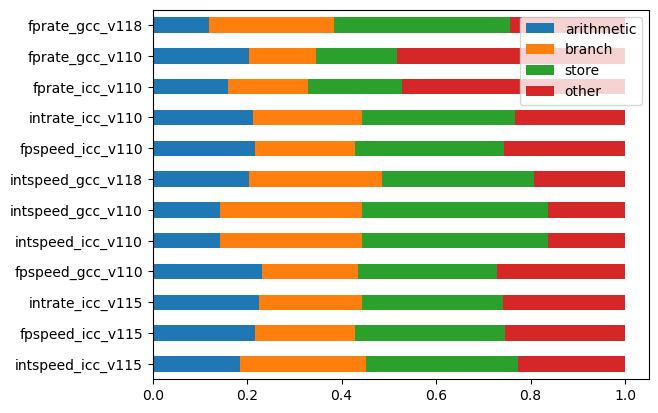
\includegraphics[width=\textwidth] {Reporte IDI-2 ITESO/img/characterization_spec.png}
    \caption{Characterization of workloads using instructions categories}
    \label{fig:char_full}
\end{figure}

\begin{figure}[h]
    \centering
    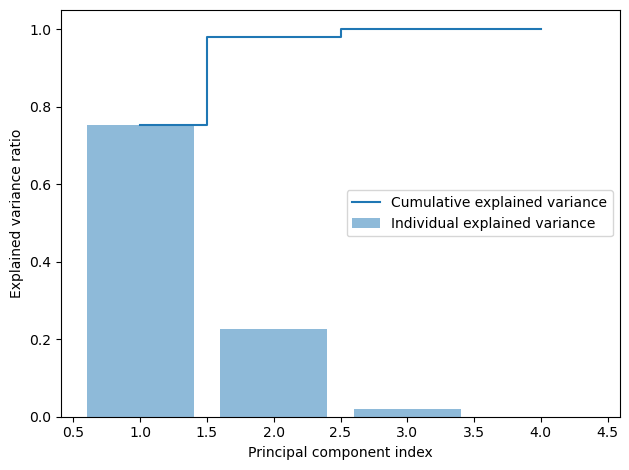
\includegraphics[width=\textwidth] {Reporte IDI-2 ITESO/img/variance_spec.png}
    \caption{Explained Variance  of workloads instructions characterization}
    \label{fig:explained_var}
\end{figure}

\begin{figure}[h]
    \centering
    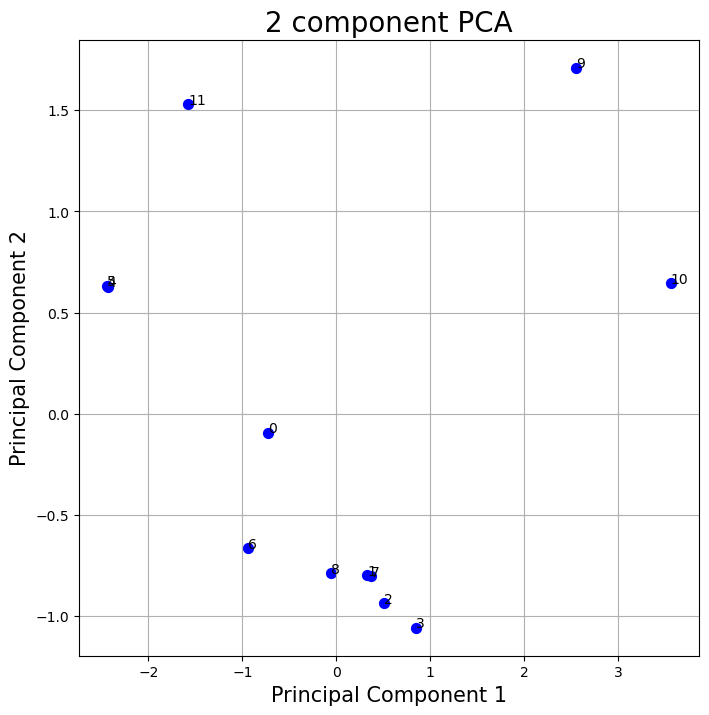
\includegraphics[width=\textwidth] {Reporte IDI-2 ITESO/img/pca_spec.png}
    \caption{Principal Component Analysis of workloads instructions characterization }
    \label{fig:pca_full}
\end{figure}

\begin{figure}[h]
    \centering
    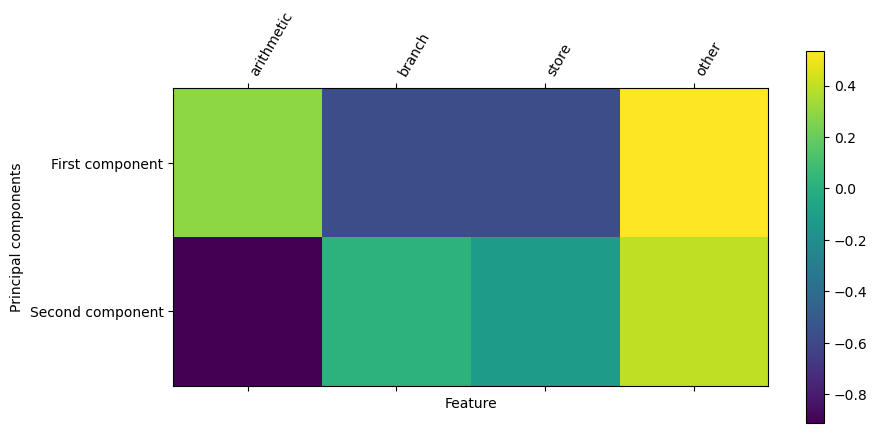
\includegraphics[width=\textwidth] {Reporte IDI-2 ITESO/img/heat_spec.png}
    \caption{ Heat map of the first two principal components on the workloads instructions histograms}
    \label{fig:heat_map}
\end{figure}

\begin{figure}[h]
    \centering
    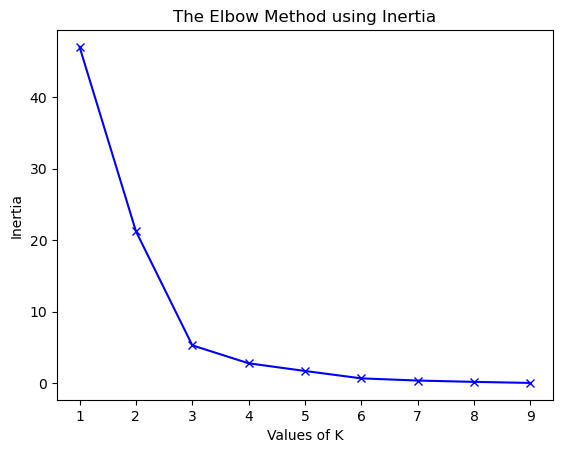
\includegraphics[width=\textwidth] {Reporte IDI-2 ITESO/img/inertia_spec.png}
    \caption{Inertia }
    \label{fig:inertia}
\end{figure}


\begin{figure}[h]
    \centering
    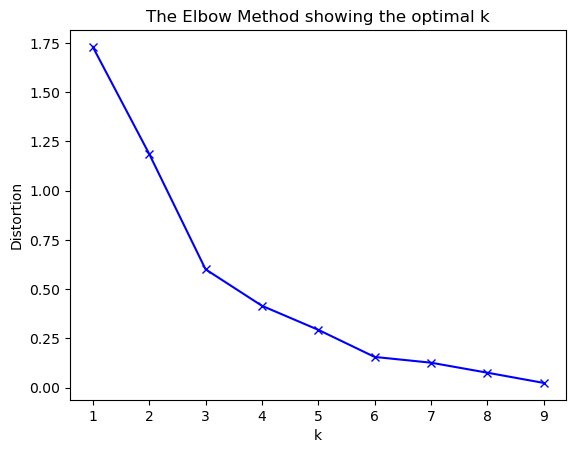
\includegraphics[width=\textwidth] {Reporte IDI-2 ITESO/img/distortion_spec.png}
    \caption{Distortion}
    \label{fig:distortion}
\end{figure}


\begin{figure}[h]
    \centering
    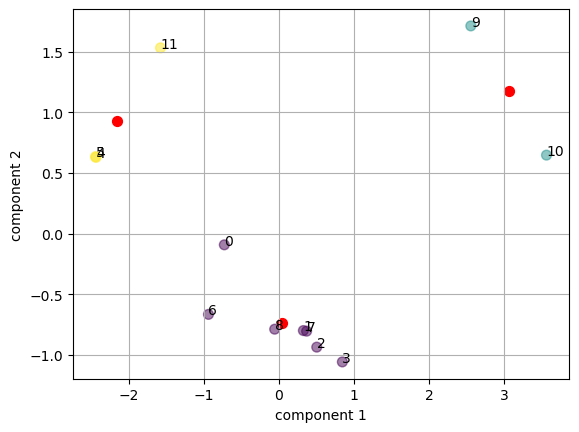
\includegraphics[width=\textwidth]{Reporte IDI-2 ITESO/img/kmean_spec.png}
    \caption{Unsupervised ML using K-mean for Instructions histograms}
    \label{fig:kmeans}
\end{figure}

\begin{figure}[h]
    \centering
    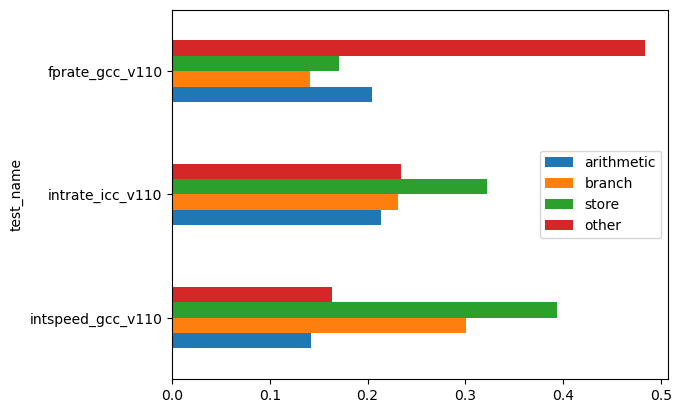
\includegraphics[width=\textwidth]{Reporte IDI-2 ITESO/img/characterization_cetroid_spec.png}
    \caption{Characteristics of tests nearest to centroid }
    \label{fig:char_small}
\end{figure}

\begin{figure}[h]
    \centering
    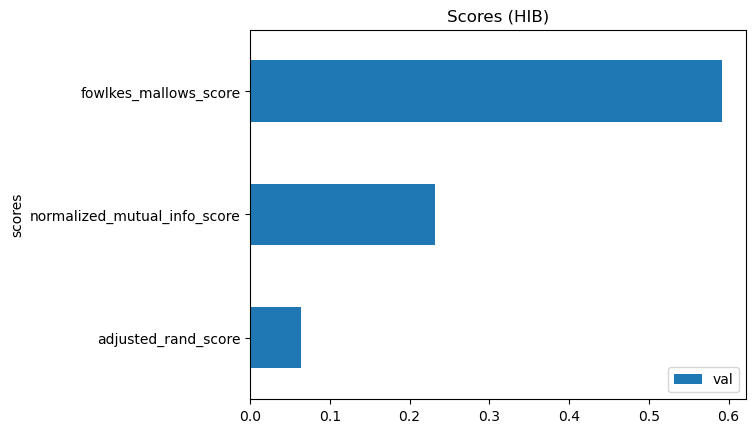
\includegraphics[width=\textwidth]{Reporte IDI-2 ITESO/img/results_spec.png}
    \caption{Accuracy of k-means classification for SpecCPU2017 workloads }
    \label{fig:results_spec}
\end{figure}



\begin{figure}[h]
    \centering
    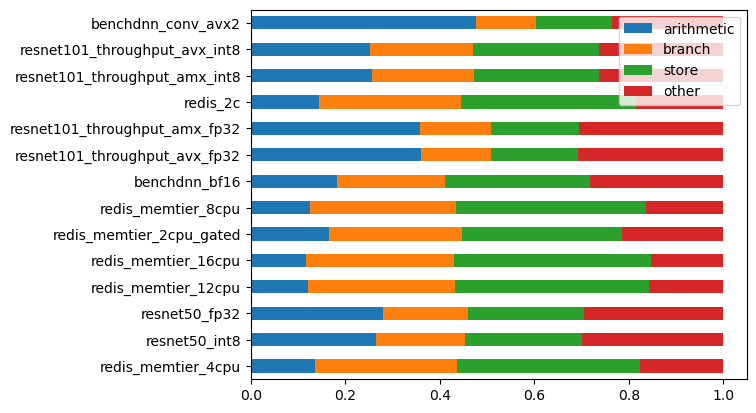
\includegraphics[width=\textwidth]{Reporte IDI-2 ITESO/img/characterization_apps.png}
    \caption{ Characterization of Resnet/Memtier/Benchdnn workloads}
    \label{fig:char_subset_apps}
\end{figure}

\begin{figure}[h]
    \centering
    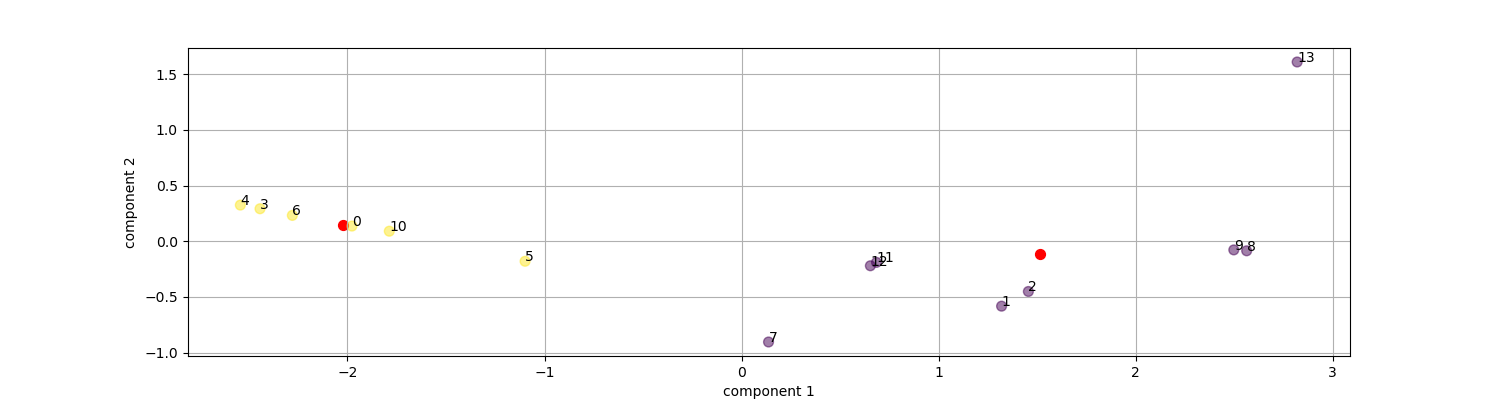
\includegraphics[width=\textwidth]{Reporte IDI-2 ITESO/img/k_means_apps.png}
    \caption{Unsupervised ML using K-mean for Instructions histograms from a subset of Resnet/Memtier/Benchdnn workloads }
    \label{fig:kmeans_apps}
\end{figure}

\begin{figure}[h]
    \centering
    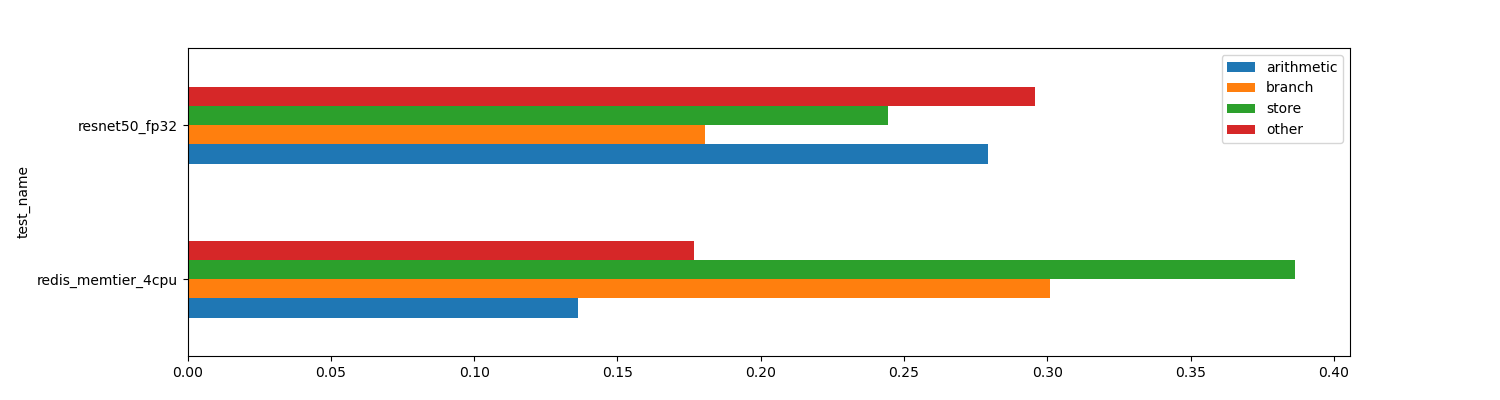
\includegraphics[width=\textwidth]{Reporte IDI-2 ITESO/img/centroid_apps.png}
    \caption{Characteristics of tests nearest to the centroid for Resnet/Memtier/Benchdnn workloads }
    \label{fig:centroid_apps}
\end{figure}

\begin{figure}[h]
    \centering
    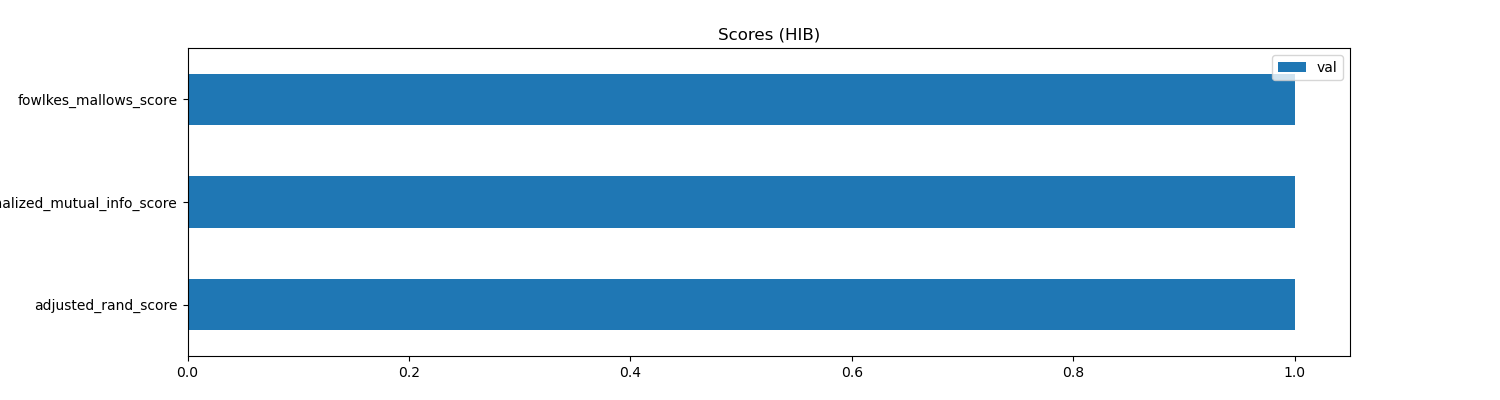
\includegraphics[width=\textwidth]{Reporte IDI-2 ITESO/img/results_apps.png}
    \caption{Accuracy of classification of ML and data base oriented applications using methodology}
    \label{fig:results_apps}
\end{figure}

\end{document}









